\documentclass{article}
\usepackage[utf8]{inputenc}
\usepackage[english, science, small]{ku-frontpage}
\usepackage{tabularx}
\usepackage{indentfirst}

\title{Software Engineering}
\subtitle{First hand-in}
\author{Matias Korn(crd551), Samuel Korn(rxq534), Nikolin Prenga (hpq143), Silvan Adrian (zlp432)}
\date{\today}

\begin{document}

\maketitle

\section{Solution and problem domain}
Citizens have the possibility to apply for loss of earnings. Loss of earnings means, that the earnings the citizen has missed out on, due to being occupied of taking care of a child. There are many actors involved when the citizen apply for loss of earnings. First off, there is the case-worker, who receives the application from the citizen. The case-worker is working at a municipality council. The municipality council has to comply with the law and paragraph 42 and the rules that are provided from the ministry of social affairs.

The ministry of social affairs lay down the rules of:
(1) How big a possible cap of allowed compensation is.
(2) How much the pension scheme is obligated to contribute with. (3) How the calculation of the actual compensation is made. (4) What the limit is of how much the pension scheme is obligated to contribute with. (5) How much of the loss on the pension contribution shall be paid by the receiver and municipal council.

As mentioned, the case-workers handles the cases and receives all the necessary information, for complying with paragraph 42. First of, the case-worker has to establish, if there are grounds for compensation. (1) The child has to be under 18. (2) The conditions on the child's health have to abide by the law, for that the child's health record has to be collected from the health care system. The health record has to confirm, that it is most expedient for the mother or father to the care of the child, at home or has been placed in care under section 52(3)(vii). If that is the case, the condition is, that it is most expedient for a parent to be there. It might be difficult to establish, if that is the case, based on the health record, if it is not explicitly stated, therefore it might be necessary to collect a confirmation by the child's doctor. (3) Loss of income has to be established, for that the necessary bank statements have to be provided.

Our solution is concerned with case management. We have to provide a platform for collecting, recording the progress and the final decisions that have been made and what grounds there has been for them. The following actors are directly involved in our system: (1) the citizen, (2) the case-worker, (3) the minister of social affairs(external system), (4) the law that decides if the citizen is permitted for loss of earnings, (5) the payment system(external system), that is available for the municipal council. Our solutions will handle the information gathering. Storing the information relevant for the case. The final decision whether or not the citizen has been granted compensation and calculating the amount granted for payout to both the citizen and pension scheme, based on the numbers provided by the minister of social affairs.

\section{Scenarios}

\subsection*{Application approved}

Alice, a parent, has a child with a serious chronic illness. She logs into the OCM system as a citizen and fills out a form, as well as attaching any relevant documentation. Once finished, she submits the application. There does not exist any prior applications from Alice, so the system annotates it as a new case.

\vspace{2mm}

The system assigns the application to caseworker Bob. He logs into the system as a caseworker. He picks Alice's application from an overview of assigned cases. He validates its authenticity. He processes the application through the system's user interface. He approves and submits the application.

\vspace{2mm}

The system assigns the application to another caseworker Charles. He processes the application in the same manner as Bob and submits it once it is approved.

\vspace{2mm}

With approvals from two random caseworkers, the system calculates the compensation based on the data contained in the application. The system sends a response to Alice's e-mail that her application was approved, including the details regarding her compensation. The system archives the application.

\subsection*{Application rejected}
\begin{enumerate}
    \item Alice, a parent, has a child with a serious fever. 
    \item Alice sends an application for "loss of earnings" through the OCM system.
    \item The system assigns the application to caseworker Bob.
    \item Bob validates the legitimacy of the application.
    \item Bob realize, that Alice's child does not meet the requirements for the illness.
    \item Bob rejects the case.
    \item Bob sends an email to Alice and informing her about the rejection and the cause. 
\end{enumerate}


\subsection*{Inquire additional information from applicant}
\begin{enumerate}
    \item Alice, a parent, has a child with a serious long-term disease.
    \item Alice sends an application for "loss of earnings" through the OCM system. 
    \item The system assigns the application to caseworker Bob.
    \item Bob validates the legitimacy of the application.
    \item Bob realize, that the application is missing a doctor confirmation. 
    \item Bob puts the case on-hold.
    \item Bob sends an email to Alice requesting a doctor confirmation.
    \item Alice provides the doctor confirmation.
    \item Bob validates the legitimacy of the application.
    \item The system calculates compensation based on data from form. 
    \item Bob approves the application.
    \item The system saves the application and any additional notes Bob has attached.
    \item The system sends a response to Alice's e-mail that her application was approved. 
\end{enumerate}

\subsection*{Illegitimate application}
\begin{enumerate}
    \item Alice, a parent, stayed home for two days because of her child had the flu. 
    \item Alice sends an application for "loss of earnings" through the OCM system.
    \item The system assigns the application to caseworker Bob.
    \item Bob approves the application, without validating the legitimacy of the application.
    \item The system saves the application and any additional notes Bob has attached.
    \item The system sends a response to Alice's e-mail that her application was approved.
\end{enumerate}

\subsection*{Duplicate application approved}

\section{Functional requirements}

% reviewing of the cases by another caseworker before processing the loss of earnings. 
% funtionelle ting som er målbare!!!!

The caseworker can make an overview of all unprocessed cases, approval cases and ongoing cases that is assigned to the caseworker. Caseworker takes an unprocessed case, approval case or pick one of his existing cases that is ongoing.

If the caseworker takes an unprocessed case, the person will be presented with all the provided documents from the applicant. If the caseworker decides the documents are falsified, he changes the status to falsified and either gets unassigned from the case or takes further action by contacting the legal authorities and provide all the necessary information, that is requested. After the falsification is handled, the case change status to prosecuted.

After the verification of the authenticity of the documents, the caseworker decides if the doctor confirmation is confirming that the legal requirements of the child's health status is met and the necessary conditions are present. 
If the conditions are not met, the application gets rejected and the caseworker can send an email directly from the system to the applicant with the  rejection and cause of the decision. 
If the documents provided does not fulfill the necessary conditions, the caseworker can send an email directly from the system to the applicant, requesting the necessary documents for further processing of the application.

When satisfactory is met and all the conditions and legal documents are met, the caseworker inputs all the relevant information to the system from the documents.

If the caseworker picks an approval case, that is not handled by the caseworker himself. The caseworker goes through all documents provided and verifies that the applicant is permitted for loss of earnings. The caseworker goes on to verify that the inputted numbers are correct.

If the caseworker decides, that the applicant is not permitted for loss of earnings, the caseworker sets the case to rejected approval. 

\section{Non-functional requirements}

\subsection{Availability}
There should be an availability of 99.99\%.

\subsection{Usability}
The software has to be easily usable.

\subsection{Accessibility}
The software should be accessible for people with disabilities. 

\subsection{Maintainability}
The software should be easily to maintain.

\subsection{Security}
The system needs to uphold the GDPR legislation.
No one should have access on data he/she has no access rights on.

\subsection{Scalability}
Should be able to be used by many concurrent users without delay.

\subsection{Language}
The software should be only available in Danish.

\subsection{Persistence}
The software has to guarantee data integrity in atleast 5 years.

\section{Use case diagram}

% to do: extend

\begin{figure}[htb!]
	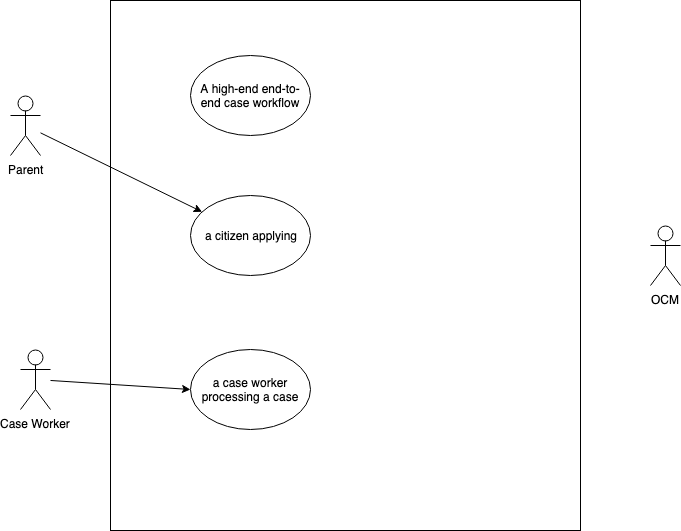
\includegraphics[width=\textwidth]{img/use-cases}
\end{figure}


\section{Detailed Use cases}

\subsection{UC01: A high-end end-to-end case workflow}

\begin{tabularx}{\textwidth}{l|l}
	\textbf{Use Case name} & A high-end end-to-end case workflow \\
	\hline
	\textbf{Participating actor} & \\
	\hline
	\textbf{Flow of events} &
	\begin{minipage}{\linewidth}
		\begin{enumerate}
			\item asds
			\item asdasdasds
		\end{enumerate} 
	\end{minipage}\\
	\hline
	\textbf{Entry condition} & \\
	\hline
	\textbf{Exit condition} & \\
	\hline
	\textbf{Quality requirements} & \\
\end{tabularx}



\subsection{UC02: A citizen applying}

\begin{tabularx}{\textwidth}{l|l}
	\textbf{Use Case name} & A high-end end-to-end case workflow \\
	\hline
	\textbf{Participating actor} & \\
	\hline
	\textbf{Flow of events} & \\
	\hline
	\textbf{Entry condition} & \\
	\hline
	\textbf{Exit condition} & \\
	\hline
	\textbf{Quality requirements} & \\
\end{tabularx}

\subsection{UC03: A case worker processing a case}
\begin{tabularx}{\textwidth}{l|l}
	\textbf{Use Case name} & A high-end end-to-end case workflow \\
	\hline
	\textbf{Participating actor} & \\
	\hline
	\textbf{Flow of events} & \\
	\hline
	\textbf{Entry condition} & \\
	\hline
	\textbf{Exit condition} & \\
	\hline
	\textbf{Quality requirements} & \\
\end{tabularx}

\subsection{UCX: ...}

\section{Architecture model}


\section{Project plan}

\subsection{Team composition/roles}
\textbf{Silvan Adrian}
\begin{itemize}
	\item SCRUM Master %otherwise won't make much sense of having a project team without a scrum master
\end{itemize}
\textbf{Matias Korn}
\begin{itemize}
	\item Developer
\end{itemize}
\textbf{Samuel Korn}
\begin{itemize}
	\item Developer
\end{itemize}
\textbf{Nikolin Prenga}
\begin{itemize}
	\item Developer
\end{itemize}

\subsection{Skill matrice}
%fill up
\begin{table}[htb!]
\begin{tabular}{lllll}
 \textbf{Skill}  & \textbf{Silvan} & \textbf{Matias} & \textbf{Samuel} & \textbf{Nikolin} \\
\hline
Development       &                 &                   &                   &                  \\
Project Management &                 &                   &                   &                  \\
                  &                 &                   &                   &                 
\end{tabular}
\end{table}

\subsection{Work Packages}
% just a graph or actually some coding involved?

\subsection{Schedule}
As the project methodology SCRUM will be used, so after each Sprint there will be  working increment released.


\begin{table}[htb!]
\begin{tabular}{lll}
\textbf{Sprint} & \textbf{Sprint Goal} & \textbf{Date} \\
\hline
1      & Set Up Infrastructure & xx.xx \\
2      & Do more etc.          &            \\
3       &                       &           
\end{tabular}
\end{table}

\subsection{Risks}

\begin{tabularx}{\textwidth}{llllXX}
\textbf{Nr} & \textbf{Description} & \textbf{Probability} & \textbf{Criticality} & \textbf{Prevention}                                                      & \textbf{Measure}                                                                             \\
\hline
R1          & Worker gets sick     & 10\%                 & high                 & Every worker should be able to replace the skill of an other in the team & Split up work not only according to someones skills but also to get them to learn new things \\
            &                      &                      &                      &                                                                          &                                                                                              \\
            &                      &                      &                      &                                                                          &                                                                                             
\end{tabularx}


\end{document}
